\chapter{CONCEITOS FUNDAMENTAIS} \label{conceitos}

Neste capitulo serão abordados todos os conceitos utilizados na realização deste trabalho, como Jogos Digitais, ferramentas para desenvolvimento destes jogos, sistemas sensíveis a contexto, o que são sinais neurais, loop de biofeedback etc. \todo{completar este capitulo com todos os principais conceitos utilizados ao desenrolar do projeto. aprendizado de máquina, métricas de avaliação, base de dados}

\section{Jogos Digitais}
Jogos digitais são aplicações interativas utilizadas como entretenimento. Esses jogos podem ser apresentados em diversas mídias: desde os conhecidos fliperamas e consoles de mesa \cite{batista2018estudo}, até os jogados em computadores e smartphones nos dias de hoje. No contexto deste trabalho, foram considerados apenas os jogos de computador como uma plataforma de testes para o algoritmo de interpretação de sinais/emoções.

\section{Game Engine}
Game engine, também conhecido como Motor Gráfico, é um framework de criação de jogos. Esses frameworks são utilizados para facilitar a criação de jogos eletrônicos, já que sua maioria possuem ferramentas agregadas a códigos já prontos de gráficos 2D/3D, simulação de física, desenvolvimento multi-plataforma, comandos I/O, sons e outros sistemas e módulos que, sem o uso de um framework, precisariam ser implementados um a um, poupando muito tempo de desenvolvimento \cite{gameengine}. Grandes desenvolvedoras costumam construir suas próprias Game Engines, mas essas costumam não ser disponibilizadas para o público geral. Para isso, também existem Game Engines públicas, como a Unity \cite{Unitysite}, que é gratuita e utilizada por milhares de usuários no mundo todo para criação de jogos, sendo a escolhida para a realização deste trabalho.

\subsection{Game Engine - Unity}
A plataforma Unity é uma ferramenta de desenvolvimento de jogos 2D e 3D baseada em C\# e estrutura de programação baseada em scripts, oferecendo diversos recursos para facilitação do trabalho de desenvolvedores desse tipo de projeto. Ela é um suporte para todos os recursos necessário no desenvolvimento de jogos digitais, como gráficos, áudio, controles e compatibilidade com diversos dispositivos.
A escolha da Unity se dá pela facilidade de encontrar elementos e projetos para se ter como base, por ser uma engine popular e gratuita, bem como pela experiência já adquirida por sua utilização no decorrer do curso.

\section{Sinais Neurais}
Sinais Neurais são pequenos impulsos nervosos realizados pelas células neurais individuais, sinais esses que são inicialmente transmitidos de maneira elétrica e passam por um processo de conversão para se tornarem químicos. Através de sistemas como o (EEG), ou Eletroencefalograma, podemos registrar os sinais emitidos assim como suas mudanças nas atividades cerebrais durante a execução de diferentes tarefas como pensar, se comunicar ou pegar um objeto, sendo possível a retirada de informações como a analise e interpretação desses impulsos nervosos e seus padrões nas atividades cerebrais, podendo assim ser realizada a investigação de deficiências neurais, estados mentais, sono e comunicação do individuo \cite{rocha2022analise}.

\begin{figure}[h]
    \centering
    \caption{Estrutura de uma célula neuronal realizando uma atividade sináptica.}
    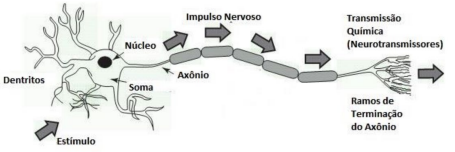
\includegraphics[width=12cm]{Figuras/celula-neural.png}
    \caption*{Fonte: \cite{rocha2022analise}}
    \label{fig:celula_neural}
\end{figure}

\section{Sistemas Sensíveis a Contexto}
Sistemas Sensíveis a Contexto são sistemas que utilizam de pistas contextuais para adaptar-se a alguma necessidade de elementos em seu ambiente. Essas pistas contextuais podem ser dados de ambiente, variáveis dinâmicas que mudam ao executar do programa ou qualquer tipo de informação que seja útil para definir características e comportamentos num cenário \cite{vieira2009modelos}. No âmbito deste projeto, o contexto ao qual o sistema será sensível é a externalização emocional do jogador, que influenciará como o próprio jogo age e reage em seu ambiente.

\section{Loop de biofeedback}
No contexto de medicina, para citar o trabalho do Dr. Michael G. McKEE na área de terapia, 
\textit{"O biofeedback envolve o monitoramento e uso de informações fisiológicas para ensinar os pacientes a modificar funções fisiológicas específicas"}\cite{biofeedback2008biofeedback}. No contexto do nosso projeto, o biofeedback participa de um círculo de interpretação e comportamento. Através dos sinais do jogador, o jogo irá adaptar-se e mudar o modo com que interage com o jogador. Com isso, o jogador tem a oportunidade de tentar controlar esses sinais afim de aproveitar melhor de um aspecto ou outro de uma mecânica. 

\section{Computação Afetiva}
Com o uso massivo de bases de dados e experimentos com o uso de inteligencias artificiais para uma interação mais humana. O termo Computação Afetiva explora justamente o comportamento das interações Humano-computador, ou seja, o modo como as maquinas podem reconhecer, interpretar e influenciar um sentimento humano. Em relação a área de jogos, o artigo \cite{filipa2019emovere} mostra a possibilidade de criar o desenvolvimento de estratégias afim de experiencias mais envolventes e personalizadas para cada jogador, onde o jogo responda ao estado emocional atual do jogador, adaptando historia, recompensas e mecânicas para determinada parte do jogo, deixando a experiência mais imersiva e satisfatória.

\break
\section{Emoções por Nível de Excitação e Valência}

 \begin{figure}[h]
    \centering
    \caption{Diagrama de Emoção por nível de Excitação e Valência}
    \centering
    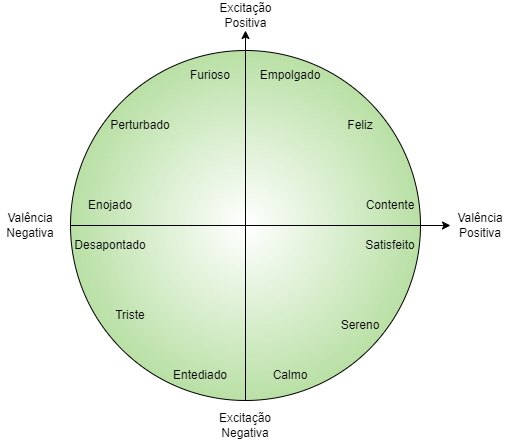
\includegraphics[width=0.5\textwidth]{Figuras/diagrama-emocional.drawio.png}
    \caption*{Fonte: Autores}
    \label{fig:diagrama_emocional}
\end{figure}

Utilizando aparelhos de medição de atividade tanto neurológica quanto fisiológica, é possível medir o nível de estresse, nervosismo ou ansiedade de uma pessoa. Cruzando esses dados com os obtidos através de uma entrevista de feedback, é possível dizer em qual direção estava apontado seu vetor emocional dentro do diagrama de excitação-valência.

